

\tikzset{every picture/.style={line width=0.75pt}} %set default line width to 0.75pt        

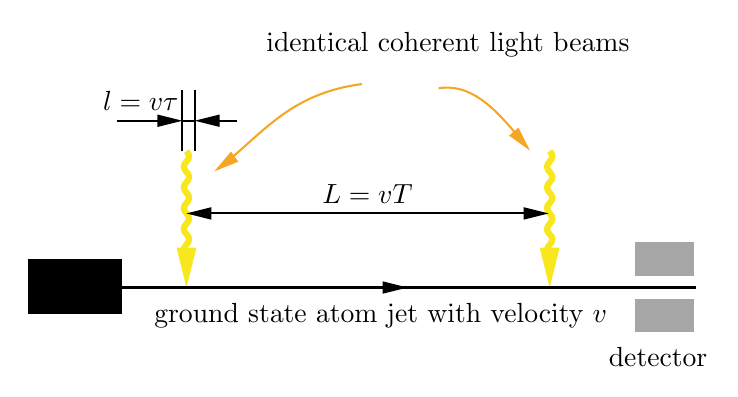
\begin{tikzpicture}[x=0.75pt,y=0.75pt,yscale=-1,xscale=1]
%uncomment if require: \path (0,300); %set diagram left start at 0, and has height of 300

%Straight Lines [id:da51441218283759] 
\draw [color={rgb, 255:red, 248; green, 231; blue, 28 }  ,draw opacity=1 ][line width=2.25]    (107,86) .. controls (108.67,87.67) and (108.67,89.33) .. (107,91) .. controls (105.33,92.67) and (105.33,94.33) .. (107,96) .. controls (108.67,97.67) and (108.67,99.33) .. (107,101) .. controls (105.33,102.67) and (105.33,104.33) .. (107,106) .. controls (108.67,107.67) and (108.67,109.33) .. (107,111) .. controls (105.33,112.67) and (105.33,114.33) .. (107,116) .. controls (108.67,117.67) and (108.67,119.33) .. (107,121) .. controls (105.33,122.67) and (105.33,124.33) .. (107,126) .. controls (108.67,127.67) and (108.67,129.33) .. (107,131) .. controls (105.33,132.67) and (105.33,134.33) .. (107,136) -- (107,137.69) -- (107,145.69) ;
\draw [shift={(107,151.69)}, rotate = 270] [fill={rgb, 255:red, 248; green, 231; blue, 28 }  ,fill opacity=1 ][line width=0.08]  [draw opacity=0] (19.2,-4.8) -- (0,0) -- (19.2,4.8) -- cycle    ;
%Straight Lines [id:da7662175680694188] 
\draw [color={rgb, 255:red, 248; green, 231; blue, 28 }  ,draw opacity=1 ][line width=2.25]    (282,86) .. controls (283.67,87.67) and (283.67,89.33) .. (282,91) .. controls (280.33,92.67) and (280.33,94.33) .. (282,96) .. controls (283.67,97.67) and (283.67,99.33) .. (282,101) .. controls (280.33,102.67) and (280.33,104.33) .. (282,106) .. controls (283.67,107.67) and (283.67,109.33) .. (282,111) .. controls (280.33,112.67) and (280.33,114.33) .. (282,116) .. controls (283.67,117.67) and (283.67,119.33) .. (282,121) .. controls (280.33,122.67) and (280.33,124.33) .. (282,126) .. controls (283.67,127.67) and (283.67,129.33) .. (282,131) .. controls (280.33,132.67) and (280.33,134.33) .. (282,136) -- (282,137.69) -- (282,145.69) ;
\draw [shift={(282,151.69)}, rotate = 270] [fill={rgb, 255:red, 248; green, 231; blue, 28 }  ,fill opacity=1 ][line width=0.08]  [draw opacity=0] (19.2,-4.8) -- (0,0) -- (19.2,4.8) -- cycle    ;
%Straight Lines [id:da2383040495531039] 
\draw    (74.5,151.69) -- (352.5,151.69) ;
\draw [shift={(213.5,151.69)}, rotate = 180] [fill={rgb, 255:red, 0; green, 0; blue, 0 }  ][line width=0.08]  [draw opacity=0] (12,-3) -- (0,0) -- (12,3) -- cycle    ;
%Straight Lines [id:da8650147298236577] 
\draw    (105,86) -- (105,56.69) ;
%Straight Lines [id:da3799472249470688] 
\draw    (111,86) -- (111,56.69) ;
%Straight Lines [id:da7976983986692758] 
\draw    (105,71.34) -- (111,71.34) ;
%Straight Lines [id:da39476271636994875] 
\draw    (113,71.34) -- (131.5,71.34) ;
\draw [shift={(111,71.34)}, rotate = 0] [fill={rgb, 255:red, 0; green, 0; blue, 0 }  ][line width=0.08]  [draw opacity=0] (12,-3) -- (0,0) -- (12,3) -- cycle    ;
%Straight Lines [id:da05730624651790883] 
\draw    (73.5,71.34) -- (103,71.34) ;
\draw [shift={(105,71.34)}, rotate = 180] [fill={rgb, 255:red, 0; green, 0; blue, 0 }  ][line width=0.08]  [draw opacity=0] (12,-3) -- (0,0) -- (12,3) -- cycle    ;
%Shape: Rectangle [id:dp9609421835293179] 
\draw  [draw opacity=0][fill={rgb, 255:red, 0; green, 0; blue, 0 }  ,fill opacity=0.35 ] (323,129.71) -- (351.5,129.71) -- (351.5,146) -- (323,146) -- cycle ;
%Shape: Rectangle [id:dp14743106980136078] 
\draw  [draw opacity=0][fill={rgb, 255:red, 0; green, 0; blue, 0 }  ,fill opacity=0.35 ] (323,157) -- (351.5,157) -- (351.5,173.29) -- (323,173.29) -- cycle ;
%Shape: Rectangle [id:dp48739879197409763] 
\draw  [color={rgb, 255:red, 0; green, 0; blue, 0 }  ,draw opacity=1 ][fill={rgb, 255:red, 0; green, 0; blue, 0 }  ,fill opacity=1 ] (31,138.69) -- (75.3,138.69) -- (75.3,164) -- (31,164) -- cycle ;
%Straight Lines [id:da7004524085571604] 
\draw    (109,116) -- (279.5,116) ;
\draw [shift={(281.5,116)}, rotate = 180] [fill={rgb, 255:red, 0; green, 0; blue, 0 }  ][line width=0.08]  [draw opacity=0] (12,-3) -- (0,0) -- (12,3) -- cycle    ;
\draw [shift={(107,116)}, rotate = 0] [fill={rgb, 255:red, 0; green, 0; blue, 0 }  ][line width=0.08]  [draw opacity=0] (12,-3) -- (0,0) -- (12,3) -- cycle    ;
%Curve Lines [id:da12367316584764931] 
\draw [color={rgb, 255:red, 245; green, 166; blue, 35 }  ,draw opacity=1 ]   (191.5,53.69) .. controls (155.73,58.28) and (143.01,78.84) .. (121.81,94.72) ;
\draw [shift={(120.5,95.69)}, rotate = 323.97] [fill={rgb, 255:red, 245; green, 166; blue, 35 }  ,fill opacity=1 ][line width=0.08]  [draw opacity=0] (12,-3) -- (0,0) -- (12,3) -- cycle    ;
%Curve Lines [id:da3353753608603731] 
\draw [color={rgb, 255:red, 245; green, 166; blue, 35 }  ,draw opacity=1 ]   (228.5,55.69) .. controls (246.84,52.79) and (259.58,70.38) .. (271.24,84.2) ;
\draw [shift={(272.5,85.69)}, rotate = 229.4] [fill={rgb, 255:red, 245; green, 166; blue, 35 }  ,fill opacity=1 ][line width=0.08]  [draw opacity=0] (12,-3) -- (0,0) -- (12,3) -- cycle    ;

% Text Node
\draw (85,67.94) node [anchor=south] [inner sep=0.75pt]    {$l = v \tau$};
% Text Node
\draw (309,179) node [anchor=north west][inner sep=0.75pt]   [align=left] {detector};
% Text Node
\draw (194.25,112.6) node [anchor=south] [inner sep=0.75pt]    {$L = v T$};
% Text Node
\draw (90,158) node [anchor=north west][inner sep=0.75pt]   [align=left] {ground state atom jet with velocity $\displaystyle v$};
% Text Node
\draw (144,27) node [anchor=north west][inner sep=0.75pt]   [align=left] {identical coherent light beams};


\end{tikzpicture}
